% --------------------------------------------------------------------------------

\begin{exercise}

Wir können einen Heap bauen, indem wir wiederholt die in der Vorlesung kennengelernte Prozedur EUNFÜGEN aufrufen, um ein Element in den Heap einzufügen.
Betrachten Sie die wie folgt geänderte ERZEUGE-HALDE-Prozedur: \\

\begin{algorithmic}
    \State ERZEUGE-HALDE'($A$)
    \State $A.\text{heap-size}:= 1$
    \For{$i = 2 ~\text{to}~ A.\text{länge}$}
        \State $\text{EUNFÜGEN}(A, A[i])$
    \EndFor
\end{algorithmic}

\begin{enumerate}[label = \alph*]

    \item Erzeugen die Prozeduren ERZEUGE-HALDE und ERZEUGE-HALDE' immer denselben Heap, wenn sie auf das gleiche Eingabefeld angewendet werden?
    (Beweis oder Gegenbeispiel)

    \item Zeigen Sie, dass ERZEUGE-HALDE' im worst case eine Laufzeit von $\Theta(n \log n)$ benötigt, um einen Heap mit $n$ Elementen zu erzeugen.

\end{enumerate}

\end{exercise}

% --------------------------------------------------------------------------------

\begin{solution}

\phantom{}

\includegraphicsboxed{DGA/DGA - Algorithmus 20 - Einfügen in eine Prioritätswarteschlange.png}
\includegraphicsboxed{DGA/DGA - Algorithmus 23 - Haldensortieren (engl. heapsort).png}

\begin{enumerate}[label = \alph*]

    \item Die beiden Prozeduren erzeugen nicht immer denselben Heap.
    Wir betrachten das Gegenbeispiel $A := [1, 2, 3]$. \\

    ERZEUGE-HALDE'($A$)

    \begin{center}
        
        \begin{tikzpicture}

            \begin{scope}[yshift = 0 cm]
                
                \draw (0, 0) node {$\mapsto$};
    
                \begin{scope}[xshift = 2 cm]
                    \filldraw [fill = white] (0, 0) circle (10 pt) node {$1$};
                \end{scope}
        
                \draw (4, 0) node {$\mapsto$};
        
                \begin{scope}[xshift = 6 cm]
                    \draw (-1, -1) -- (0, 0);
                    \filldraw [fill = white] (0, 0) circle (10 pt) node {$1$};
                    \filldraw [fill = white] (-1, -1) circle (10 pt) node {$2$};
                \end{scope}
        
                \draw (8, 0) node {$\mapsto$};
        
                \begin{scope}[xshift = 10 cm]
                    \draw (-1, -1) -- (0, 0);
                    \filldraw [fill = white] (0, 0) circle (10 pt) node {$2$};
                    \filldraw [fill = white] (-1, -1) circle (10 pt) node {$1$};
                \end{scope}
    
            \end{scope}

            \begin{scope}[yshift = -3 cm]

                \draw (0, 0) node {$\mapsto$};
    
                \begin{scope}[xshift = 2 cm]
                    \draw (-1, -1) -- (0, 0);
                    \draw (1, -1) -- (0, 0);
                    \filldraw [fill = white] (0, 0) circle (10 pt) node {$2$};
                    \filldraw [fill = white] (-1, -1) circle (10 pt) node {$1$};
                    \filldraw [fill = white] (1, -1) circle (10 pt) node {$3$};
                \end{scope}
        
                \draw (4, 0) node {$\mapsto$};
        
                \begin{scope}[xshift = 6 cm]
                    \draw (-1, -1) -- (0, 0);
                    \draw (1, -1) -- (0, 0);
                    \filldraw [fill = white] (0, 0) circle (10 pt) node {$3$};
                    \filldraw [fill = white] (-1, -1) circle (10 pt) node {$1$};
                    \filldraw [fill = white] (1, -1) circle (10 pt) node {$2$};
                \end{scope}

            \end{scope}
    
        \end{tikzpicture}

    \end{center}
    
    ERZEUGE-HALDE($A$)

    \begin{center}
        
        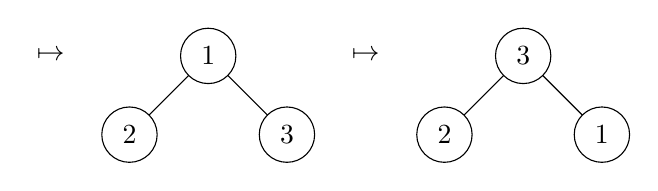
\begin{tikzpicture}
    
            \draw (0, 0) node {$\mapsto$};

            \begin{scope}[xshift = 2 cm, yshift = 0 cm]
                \draw (-1, -1) -- (0, 0);
                \draw (1, -1) -- (0, 0);
                \filldraw [fill = white] (0, 0) circle (10 pt) node {$1$};
                \filldraw [fill = white] (-1, -1) circle (10 pt) node {$2$};
                \filldraw [fill = white] (1, -1) circle (10 pt) node {$3$};
            \end{scope}
    
            \draw (4, 0) node {$\mapsto$};
    
            \begin{scope}[xshift = 6 cm, yshift = 0 cm]
                \draw (-1, -1) -- (0, 0);
                \draw (1, -1) -- (0, 0);
                \filldraw [fill = white] (0, 0) circle (10 pt) node {$3$};
                \filldraw [fill = white] (-1, -1) circle (10 pt) node {$2$};
                \filldraw [fill = white] (1, -1) circle (10 pt) node {$1$};
            \end{scope}
    
        \end{tikzpicture}

    \end{center}

    \item Die \textbf{for}-Schleife in der Angabe sorgt dafür, dass EUNFÜGEN $(n-1)$-mal ausgeführt wird.
    Der Einfachheit halber sei dies aber $n$.

    EUNFÜGEN führt eine Aufwärts-Korrektur der aktuellen Halde an dem letzten Knoten im Datenfeld durch.
    Wenn man die Halde als Binärbaum auffasst, ist das immer der unterste, rechteste Knoten.
    Aufwärts-Korrektur springt immer von Sohn zu Vater, insgesamt muss also die gesamte Tiefe $\ceil{\log_2 i}$ des aktuellen Binärbaums mit $i = 1, \dots, n$ Knoten raufgesprungen werden.

    \begin{multline*}
        \Omega(n \log n)
        =
        \frac{n}{2} (\log_2 n - \log_2 2)
        =
        \frac{n}{2} \log_2 \frac{n}{2}
        =
        \log_2 \pbraces{\frac{n}{2}}^\frac{n}{2}
        \stackrel{!}{\leq}
        \log_2 n!
        =
        \log_2 \prod_{i=1}^n i
        =
        \sum_{i=1}^n \log_2 i \\
        \leq
        T(n)
        :=
        \sum_{i=1}^n \ceil{\log_2 i}
        \leq
        \sum_{i=1}^n (\log_2 n + 1)
        =
        n \log_2 n + n
        =
        \Landau(n \log n)
    \end{multline*}

    Die Ungleichung mit dem \enquote{!} kommt aus der Vorlesung.
    Mit den beiden Abschätzungen erhalten wir nun für die Laufzeit $T(n) = \Theta(n \log n)$.

\end{enumerate}

\end{solution}
